\documentclass[titlepage]{article}

\usepackage[margin=1in]{geometry}
\usepackage{fancyhdr}
\usepackage{csquotes}
\usepackage{marginnote}
\usepackage{scrextend}
\usepackage[bottom]{footmisc}
\usepackage{enumitem}
\usepackage{amsmath,amssymb,amsthm}
\usepackage{mathtools,physics}
\usepackage{tikz}
\usepackage{pdfpages}
\usepackage[hidelinks]{hyperref}

\fancypagestyle{main}{
    \fancyhf{}
    \fancyhead[L]{\leftmark}
    \fancyhead[R]{MATH 16110}
    \fancyfoot[R]{Labalme \thepage}
}

\MakeOuterQuote{"}

\reversemarginpar

\deffootnotemark{\textsuperscript{\textup{[}\thefootnotemark\textup{]}}}
\deffootnote[2.1em]{0em}{0em}{\textsuperscript{\thefootnote}}

\setenumerate[itemize,3]{label={\scriptsize$\blacksquare$}}

\setcounter{secnumdepth}{0}

\newcommand{\N}{\mathbb{N}}

\title{MATH 16110 (Honors Calculus I IBL) Notes}
\author{Steven Labalme}

\begin{document}




\maketitle



\pagenumbering{roman}
\tableofcontents
\newpage



\pagenumbering{arabic}
\pagestyle{main}
\renewcommand{\sectionmark}[1]{\markboth{#1}{}}
\section{Introduction to Proofs}
\begin{itemize}
    \item \marginnote{9/27:}Note: These answers address the exercises on the following document.
    \item We will prove Lemma 4 (i) by contrapositive.
    \begin{proof}
        We wish to prove that if $x$ and $y$ are not both odd, then $xy$ is not odd. In other words, we wish to prove that if at least one of $x$ or $y$ is even, then $xy$ is even. Let's begin. Let $x$ be even. Then $x=2k$ for some $k\in\N$. Thus, $xy=2(ky)$, proving that $xy$ is even since $ky\in\N$. A similar argument holds if we first let $y$ be even.
    \end{proof}
    \item We now prove Corollary 5.
    \begin{proof}
        We wish to prove that $xy$ is even if and only if at least one of $x$ and $y$ is even. Consequently, we must prove the dual implications "if $xy$ is even, then at least one of $x$ and $y$ is even" and "if at least one of $x$ and $y$ is even, then $xy$ is even." Let's begin. For the first statement, let $xy$ be even and suppose for the sake of contradiction that and both $x$ and $y$ are odd. But by Lemma 4, it follows from the assumption that $x$ and $y$ are both odd that $xy$ is odd, a contradiction. Therefore, at least one of $x$ or $y$ must be even. As to the second statement, see the proof of Lemma 4.
    \end{proof}
    \item Are there positive integers $m,n$ such that $m$ and $n$ have no common factors (other than 1) and $m^2=3n^2$? Either give an example or prove that no example is possible.
    \begin{proof}
        Let $m,n$ be relatively prime positive integers and suppose for the sake of contradiction that $m^2=3n^2$. We divide into two cases. If $n$ is even, then $3n^2=3(2k)^2=12k^2=2(6k^2)=m^2$ where $k\in\N$, proving that $m^2$ is even. By Corollary 5, this implies that $m$ is even. Therefore, since $m$ and $n$ are both even, they have a common factor, a contradiction. On the other hand, if $n$ is odd, then $3n^2=3(2k+1)^2=12k^2+12k+3=2(6k^2+6k+1)+1=m^2$ where $k\in\N$, proving that $m^2$ is odd. Thus, by Lemma 4, $m$ is odd. Then $m^2=(2l+1)^2=4l^2+4l+1=12k^2+12k+3$, which implies that $2(l^2+l)=2(3k^2+3k)+1$, i.e., that an odd number equals an even number, a contradiction. Hence, in both cases, we must have that $m^2\neq 3n^2$.
    \end{proof}
    \item Are there positive integers $m,n$ such that $m$ and $n$ have no common factors (other than 1) and $m^2=6n^2$? Either give an example or prove that no example is possible.
    \begin{proof}
        Let $m,n\in\N$ have no common factors (other than 1), and suppose for the sake of contradiction that $m^2=6n^2$. Since $6n^2=2(3n^2)=m^2$, $m^2$ is even. It follows by Corollary 5 that $m$ is even. Thus, $m^2=4k^2=6n^2$, so $2k^2=3n^2$. Consequently, $3n^2$ is even. Then by Corollary 5 again, we have that $n^2$ is even (since at least one of 3 or $n^2$ is even and 3 is odd). By Corollary 5 one more time, $n$ is even. Thus, $m$ and $n$ are both even, contradicting the assumption that they have no common factors other than 1.
    \end{proof}
    \item Are there positive integers $m,n$ such that $m$ and $n$ have no common factors (other than 1) and $m^2=4n^2$? Either give an example or prove that no example is possible.
    \begin{proof}
        Let $m=2$ and $n=1$. Then $m^2=2^2=4=4\cdot 1^2=4n^2$.
    \end{proof}
\end{itemize}

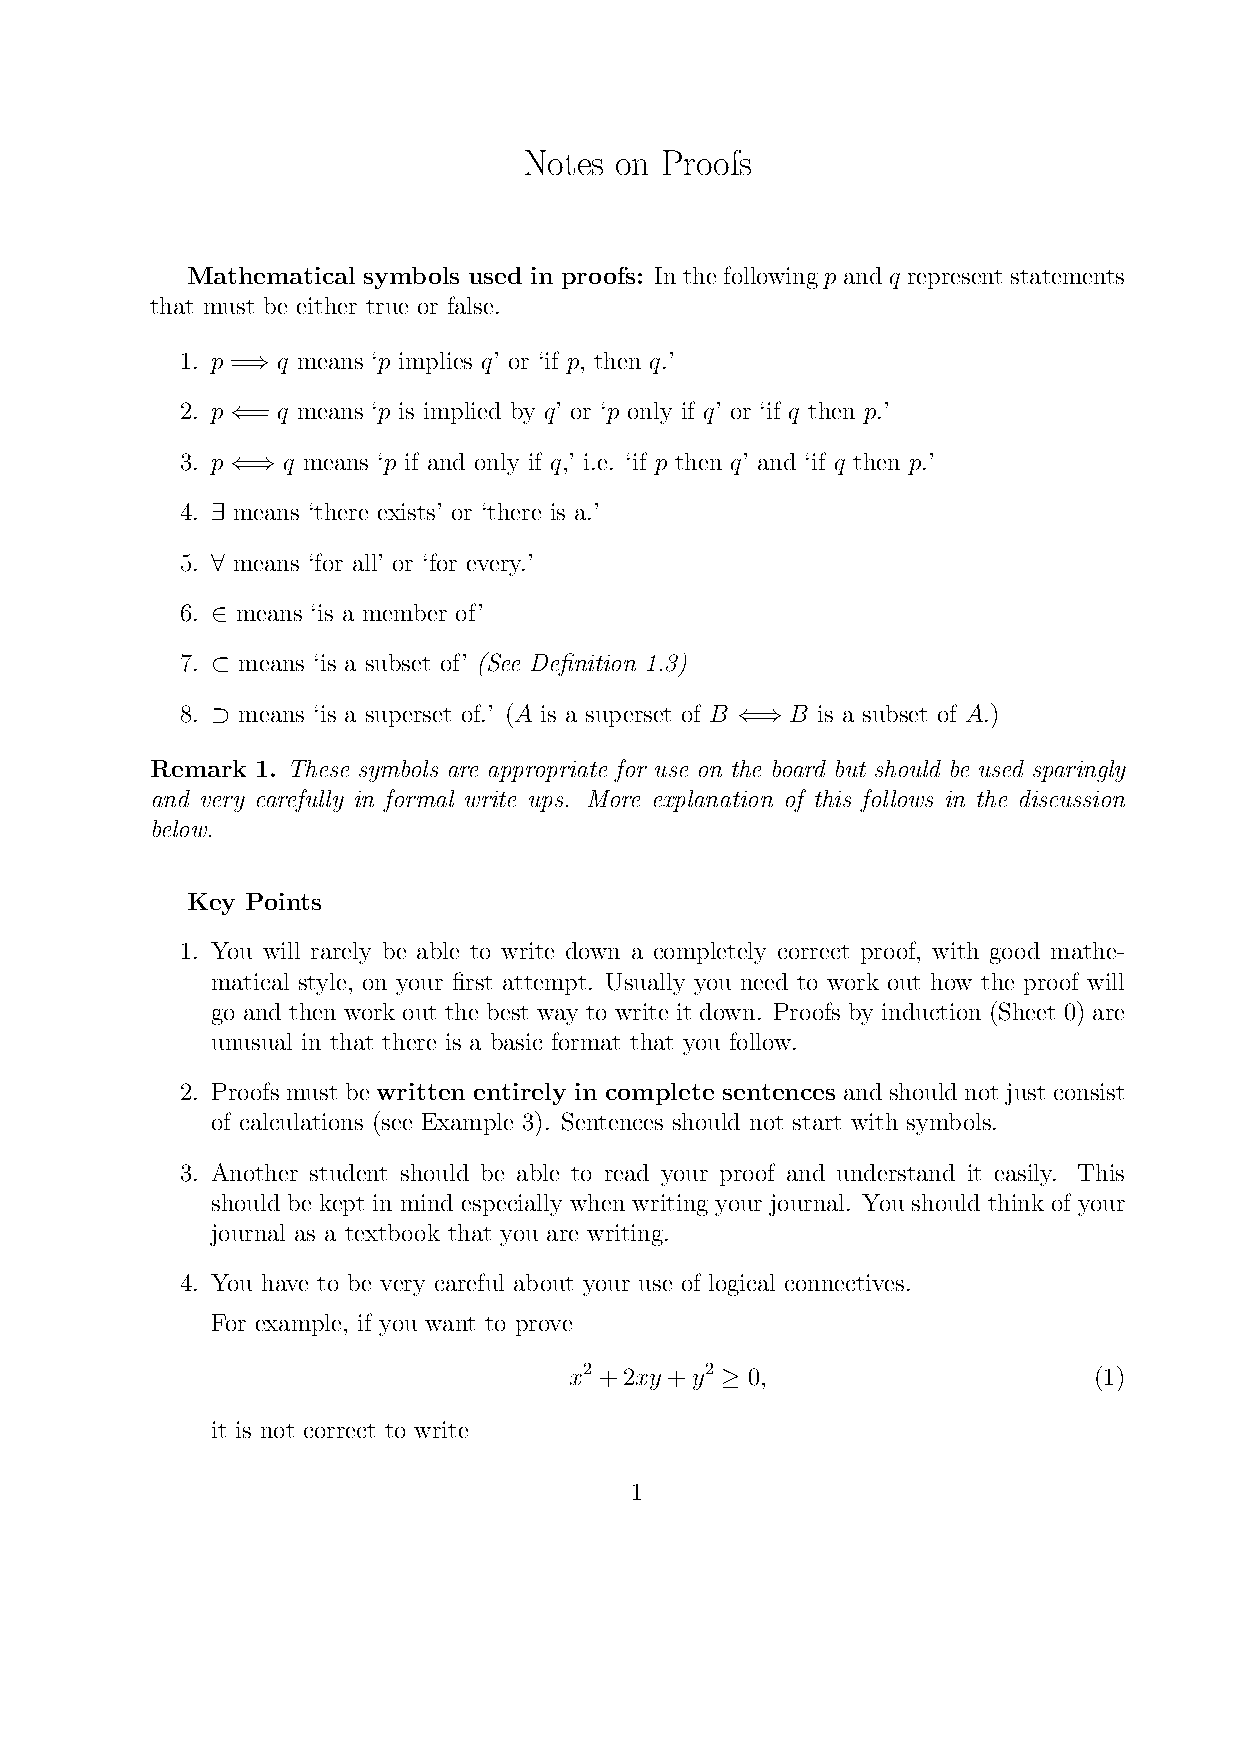
\includepdf[pages=-]{PDFs/WhatIsAMathematicalProof}




\end{document}